% !TEX root = ../thesis.tex
%
\chapter{Implementation Details}
\label{sec:implementation}

Besides the theoretical basics presented in \Cref{sec:related} the \gls{tessla} runtime of this thesis is built upon a number of technologies.
To better understand decisions made during the implementation this chapter will give an overview of them and show why they were choosen.

As already mentioned, the implemented runtime itself is independent of the way traces are generated.
Therefore we will not only look at the building blocks for the runtime itself but also examine related projects which can be used to obtain traces, which then can be monitored by the runtime.
Because the format of the traces can differ heavily, depending on how and why they were collected, they are not only used to test the runtime but also to determine how the runtime can consume them.

\section{TesslaServer}
\label{sec:implementation:tesslaserver}

The runtime to evaluate specifications against traces is implemented in the programming language Elixir, which itself is built on top of Erlang, the \gls{beam} \gls{vm} and \gls{otp}.
To understand why this platform was choosen we will look at the Erlang ecosystem in the next section.
Note that in the following sections terminology from \Cref{sec:related,sec:definitions} as well as from Erlang and Elixir is heavily used.

\subsection{Erlang and Elixir}
\label{sec:implementation:tesslaserver:erlang_elixir}

Erlang was originally developed 1987 as a language to program systems with limited resources which had to be highly fault tolerant.
The primary purpose of the language were phone switches, which have to handle large amounts of connections at the same time.
Since the switches weren't deployed at a central location but wherever they are needed crashes would entail long downtimes of the system.
Also, since customers expect permanent service, the platform had to provide a way to update the software without downtimes.
With these requirements the language and the \gls{otp} platform were developed.

While the requirements of TesslaServer are quite different we will see that the Erlang platform is a great fit for the implementation.

The rather new programming language Elixir\footnote{\url{http://elixir-lang.org}} can be seen as a dialect of Erlang.
Elixir code is compiled into bytecode for \gls{beam} and can therefore interoperate with Erlang code.
The rationale to use Elixir instead of Erlang is twofold:
On the one hand Erlangs syntax is pretty different from that of most modern general purpose programming languages while Elixirs syntax was developed based on modern language design principles.
Also Elixir supports metaprogramming, meaning you can write code that generates code at compile time, which is heavily used as described in \Cref{sec:implementation:tesslaserver:architecture}.

One of the core strengths of the Erlang platform is it support to use multiple processor cores, even if these cores are deployed over multiple machines in a network.
The platform offers tools to develop code that can be distributed over multiple processors.
This distribution is transparent to the developer.
The underlying concept of the distribution is the actor model, first introduced in \cite{Hewitt1973}.

An actor is basically a self contained entity, that holds a state and can receive and send messages to other actors.
Since an actor holds its own state and is the only one that can manipulate it, an actor can be scheduled on any core as long as the runtime guarantees transparent message delivery.
When an actor receives a message from another actor the \gls{beam} \gls{vm} will eventually schedule the code responsible for handling the message on an available core.
This code can then access the state, alter it and send a response to the sender of the message.
In this sense an actor can be seen as a state machine, which alters the state everytime it receives a message.
Since actors are independent of each other they can be scheduled in parallel on multiple processors.
Only when two actors synchronously communicate one has to wait for the other.


Another reason to choose the Erlang platform was its support for multiple plattforms, including resource restricted ones.
While this thesis only considers offline monitoring it may be a future goal to perform online monitoring with TesslaServer.
To enable this the runtime has to be able to run on the same hardware architecture the monitored program runs on sharing resources with it.
An example of the variety of the supported platforms of Erlang and Elixir is the Nerves project\footnote{\url{http://nerves-project.org}} which allows developers to build embedded software.

\subsection{Architecture}
\label{sec:implementation:tesslaserver:architecture}

As described in \Cref{sec:definitions:eval_engine} \gls{tessla} specifications form a \gls{dag} of nodes, which perform transformations on streams and send their computed streams to children nodes.
Streams can be seen as a sequence of events or changes that can be represented as messages between the nodes.
This form of specification can be easily implemented as an actor based system, where each vertex in the \gls{dag} is implemented as an actor and the communication between adjacent vertices is realised with message passing.
Interestingly this architecture enables the simulation of greedy schedules described in \Cref{def:greedy_schedule} while the Erlang runtime itself only guarantees a fair scheduling.
To understand how this work the details of message passing and handling in Erlang is important.
Basically there are two ways two Erlang processes can communicate with each other through messages: synchronous and asynchronous.
To send a message synchronous the \emph{call} \gls{api} is used.
A \emph{call} will send a message to another process and block until a response is received.
The \emph{cast} \gls{api} is the asynchronous counterpart, which will send a message and immediately passes back control to the process that used it.

It can be easily seen, that the usage of the synchronous \gls{api} will lead to a valid greedy schedule, since the sources in the \gls{dag} will have to wait for their children to finish and the children will transitively have to wait for their children.
This means that each new message gets distributed through the whole graph as fast as possible.
While this behaviour is an interesting observation the actual implementation uses the asynchronous \gls{api} to take better advantage of parallel evaluation.

An important characteristic of \gls{tessla} specifications is, that they can specify properties targeting realtime characteristics.
On the one hand this enables specifications that aren't feasible with more classical specification approaches, like \gls{ltl} or \gls{lola}, which work on synchronous streams, on the other hand it adds complexity to monitoring approaches, since it adds asynchronicity to all parts of the system.
One point where this is important is in the way, how systems have to be monitored, or more precisely how their generated events are encoded.
For synchronous monitoring approaches, the information, that an event happened is sufficient, for asynchronous ones it is important to know at which exact time each event happened.
For an implementation of an asynchronous monitoring approach this simply means, that the representation of events has to include information about the time of the event.
Another consequence of the asynchronous nature is discussed in \Cref{sec:implementation:tesslaserver:nodes} with the notion of the \emph{front} of events.

\subsection{Synthesis of the Evaluation Engine}

The first step that TesslaServer has to perform to evaluate a specification is to synthesise the evaluation engine that will consume the traces and perform the computation.
For this step a specification is compiled into a \gls{json} based format that describes the nodes and their relationship.
\Cref{listing:spec_json} shows a minimal example of the format, which includes three nodes: two literals and a node adding their value.

\lstinputlisting[float,language=json,caption={Minimal example of the \gls{json} based specification format. The specification describes a \gls{dag} with three nodes: two literals as the sources and an adder as their child.},label=listing:spec_json]{content/code/minimal.tessla}

The compiler performs multiple checks, e.g. type checks and ensures that no loops are present in the specification, and transformations, e.g. resolve macros and other syntactic elements of the specification language.
Since the compiler acts as a safety guard, TesslaServer assumes that a given specification is error free and performs no redundant safety checks.
Invalid specifications can therefore lead to all kinds of wrong behaviour if fed to TesslaServer.

The \gls{json} based specification is then translated into actors as follows: For each node described in the \(\mathit{items}\) object an actor is started with the Elixir module specified by the \(\mathit{nodetype}\) key as the message handling code.
When a node is started as an actor it will receive the additional information present in the \gls{json} object, e.g. the value for the \(\mathit{operands}\) keys, as an argument to its initialization handler.
It will use this information to build up the initial state and to register itself with a central process registry provided by erlang under its \(\mathit{id}\).

After all actors are started, TesslaServer will send each actor a message asking them to subscribe to their operands.
When a node subscribes to an operand it will send the operand a message containing the nodes \(\mathit{id}\) with the request to add this node as a child.
The node representing the operand will add the \(\mathit{id}\) the list of children in its internal state.
Later, during the actual evaluation of the traces, each node will use the list of children to send messages of new generated events using the central process registry.

The evaluation engine is synthesized, when all nodes subscribe to their operands and can start to evaluate the specification over traces.
To understand how the evaluation works, the next section will explain the implementation of nodes.

\subsection{Node Implementation}
\label{sec:implementation:tesslaserver:nodes}

\emph{Nodes} (or \emph{computations} due to namespace errors with the Erlang standard library) are responsible for the actual evaluation of a specification over traces.
\Gls{tessla} defines a standard set of nodes (called functions in the original specification) but leaves it open to the runtime to support only part of them or extend it.
To support extensions of \gls{tessla} and the runtime one of the main focuses was to make it easy to implement new node types.

This is achieved by building upon an abstraction from \gls{otp} called \emph{GenServer} and providing a new abstraction which is tailored towards implementing a node for stream transformation, called \emph{GenComputation}.
\Cref{fig:chap6:sec_node_impl:node_control_flow} shows the control flow of a single node with two inputs and one child node.

\begin{figure}
  \center
  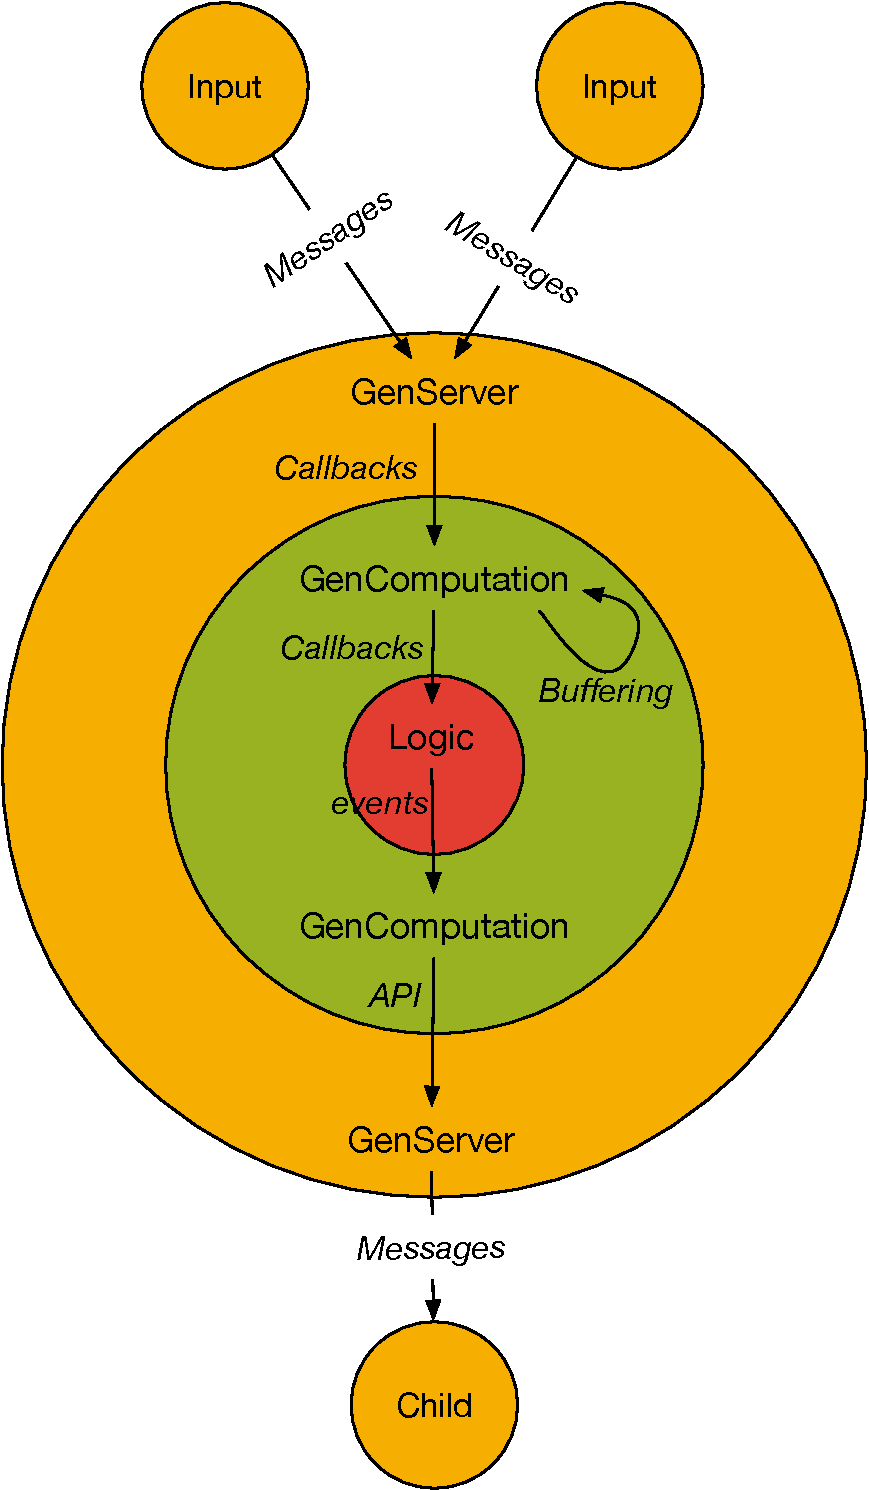
\includegraphics[width=\textwidth,height=0.9\textheight,keepaspectratio]{content/figs/node_architecture}
  \caption[Control flow of a node]{Schema of the control flow of a node. A node interacts with other nodes using the \emph{GenServer} abstraction, buffers events using the \emph{GenComputation} abstraction and performs its calculation in the \emph{logic} part. Computed events are then send to children using the same abstraction mechanisms.}
\label{fig:chap6:sec_node_impl:node_control_flow}
\end{figure}

The \emph{GenServer} abstraction is provided by the Erlang and Elixir platform and is basically an implementation of the actor pattern mentioned before.
It provides an \gls{api} to register actors, send messages to other actors and to handle incomming messages as well as maintaining the actor state.
Furthermore it enables monitoring, crash recovery and hot code upgrades, mechanism that aren't used in TesslaServer as of now.

The next layer is provided by the \emph{GenComputation} abstraction.
Before examining its responsibilities we will look at it's implementation.
\emph{GenComputation}, similar to \emph{GenServer}, heavily relies on Elixir metaprogramming, which is achieved with macros.
Elixir makes heavy use of macros, a mechanism mainly known from the LISP programming language.
Macros enables the programmer to write code that generates code.
Since all nodes perform a similar task, performing computations on one or more input streams, it makes sense to generate code for shared responsibilities instead of duplicating it for every node.
In this special case macros are used to achieve similar goals as inheritance in object oriented programming languages, namely code reuse.

Let's now focus on the responsibilities of \emph{GenComputation}.
When a node receives a message from another node, the message will be handled by the \emph{GenServer} abstraction.
\emph{GenServer} itself requires the user to implement a callback method which is responsible for actually handling a received message, e.g. by updating the state or sending new messages.
Since TesslaServer uses exactly one format for messages \emph{GenComputation} is able to handle them for all actual node implementations in a general way and only invoke actual node logic when needed.
The concrete handling of messages differs beween the two versions of TesslaServer, therefore the details are described in \Cref{sec:implementation:tesslaserver:v1,sec:implementation:tesslaserver:v2}.

On a high level \emph{GenComputation} buffers messages until it can be sure, that all inputs have progressed since the last time outputs were generated by the node, which means that either new events can be generated or at least the output stream can be progressed.
A similar concept is presented in~\cite{Hall2011} which we discussed in \Cref{sec:related:stream_based:beepbeep}: the \emph{front} of the input streams.
Because BeepBeep isn't using timed specifications the computation of the front is easy: the head of each input when every input has at least one event buffered.
For \gls{tessla} this is not as easy, since the timestamps of the events in the front can differ.
As a result \emph{GenComputation} has to perform multiple steps to determine the appropriate actions to take based on the events of the front.
The exact steps are described in the respective sections of the two versions of TesslaServer.
When \emph{GenComputation} has determined that at least one new transformation can happen it invokes the actual node logic by calling a callback method that each node has to implement.

\subsection{TesslaServer V1: Stream passing}
\label{sec:implementation:tesslaserver:v1}

The first version of TesslaServer was built with two goals in mind: safety and hiding complexity.
This led to implementation decisions that were on one hand performance critical (see \Cref{sec:evaluation:runtime_benchmarks}) and on the other hand made it hard to implement complex node types.

One of the main ideas of this implementation is to make streams a central data structure that is able to guarantee some safety aspects, e.g. ordering of events.
Each node has a set of streams: one for each parent node and one output stream.
Whenever a node computes new events, its output stream is updated and the whole stream is send to all of its children.
When a node receives a message from a parent node containing an updated stream, it will update its own state by replacing the last saved stream from the parent with the newly received.
Then it will determine if with this updated stream new events can be computed.
To do so it looks at the input stream with the minimal progress and compare it with the progress of its own output.
If theese two times are equal the node can't produce a new front, since at least one input hasn't progressed since the last computation.
Only if the minimal progress of all inputs is bigger than the progress of the output the node has to determine the appropriate computations.

This happens by generating a sequence of partial fronts for specific timestamps like following:

\begin{enumerate}
  \item Look at all input streams and find all events that happened after the progress of the output upto the minimal progress.
  \item Take the timestamps of theese events in chronological order, we will call them the \emph{change timestamps} since they denote that at least on one input stream something changed.
  \item Iterate over the timestamps in order, built partial fronts by getting all events that happened on any input stream at that timestamp.
  \item\label{sec:implementation:tesslaserver:v1:item_logic_call} Invoke the actual logic of the node for each partial front to perform its transformation.
  \item Add the generated events to the output stream and send the updated output stream to all children.
\end{enumerate}

It is important to understand, that all steps except Step \ref{sec:implementation:tesslaserver:v1:item_logic_call} are performed by the \emph{GenComputation} abstraction.
Hence, a node implementation, at least in theory, only has to implement the logic to combine a partial front to a new output.

The problems of this approach are twofold:
First, to implement more complex node types it was necessary to overwrite a lot of the provided abstractions, e.g. to manipulate timestamps.
But more important were scaling problems: Since every node had a copy of all input streams stored in its state and streams contained all events that were ever produced the \gls{ram} usage did grow exponentially with thenumber of nodes and input events used to evaluate a specification.
This can be seen in \Cref{sec:evaluation:runtime_benchmarks:num_events}.
Another problem was that the messages between nodes also grow with the number of events, since the whole stream has to be send everytime.

Therefore the TesslaServer version 2 architecture was implemented.

\subsection{TesslaServer V2: Event passing}
\label{sec:implementation:tesslaserver:v2}

The second version used the insights of the first version to provide better abstractions.
Scalability and making complex node types possible to implement were the main goals of the architecture.

To achieve theese goals some changes has to be made:
Streams are no longer an explicit data structure in the system but mere an attribute of events to denote on which stream they happened.
At the cost of some safety guarantees, which explicit streams provided, a simpler and clearer control flow of nodes and a very small \gls{api} of the new version of \emph{GenComputation} was achieved.

In the new architecture simple node types have to implement more logic, since they have to decide how to handle progress events, which became necessary in the new architecture to propagate that a stream has progressed to a new timestamp without an event happening on it.
In the old architecture the \emph{GenComputation} abstraction handled theese cases for all nodes, which wasn't appropriate for some node types.
To avoid too much code duplication a new abstraction \emph{GenLifted} is provided, which can be used as the building block for node types that \emph{lift} a function, which normaly would run on two values, to run on two signals.
This approach avoids the problems of the old architecture by moving concerns out of the base \emph{GenComputation} abstraction and making it optional to use the new \emph{GenLifted} abstraction.

The new approach to sending messages between nodes is to send each generated event as one message.
This will lead to an overall increase in messages but simplifys the handling of them.
With the new architecture nodes have a buffer for each parent node in their state.
In this buffer all events received from that parent are saved, that weren't part of a front upto that point in time.
The process of handling new messages and computing the partial fronts implemented in the new version of \emph{GenComputation} is the following:

\begin{enumerate}
  \item Add the newly received event to the end of the buffer that stores events of that parent node.
  \item Test if on each buffer at least one event is stored.
  \item End if at least one buffer has no events.
  \item Else determine the minimal timestamp over the first events of all buffers.
  \item Remove all events from the head of the buffers with that exact timestamp, they form a partial front.
  \item\label{sec:implementation:tesslaserver:v2:item_logic_call} Invoke the actual logic of the node for the partial front to perform its transformation.
  \item This will generate at least a new progress event or one or more normal events, send them to all children of the node.
  \item Go to Step 2.
\end{enumerate}

Note again how only at Step \ref{sec:implementation:tesslaserver:v2:item_logic_call} the actual node logic is invoked, meaning only that part has to be implemented for each new node type.
Nonetheless this procedure adds more responsibilities to the programmer of new node types:
In the old approach the actual node logic didn't have to handle progress events and caching of events that are important for future computations.
This can be described as the concept of making complexity explicit: The implementation has to actually handle complex edge cases in contrast to the old approach which tried to hide this complexity.

One side effect of the new implementation is that one limitation on input traces is no longer needed:
In the first implementation traces had to be totally ordered over all streams, the new implementation works as long as traces are ordered per stream.
This is especially useful when using traces that were generated by multithreaded systems: When it can be guaranteed, that each stream in the trace is exclusive to one thread, the generated trace file can be directly fed to TesslaServer.
This can easily be achieved by including an unique identifier per thread in the stream identifier.

\section{Instrumentation Pass}
\label{sec:implementation:instrumentation}

While the implementation of the actual runtime was the main goal of this thesis another project was also developed, mainly to provide test traces for the runtime.
Since this project uses some interesting technologies and can be extended to support a wide variety of trace data generation, the used technologies will be described in this chapter.

The need for a tool to generate traces arised, when no suitable test data for the runtime could be found.
As reasoned in \Cref{sec:related:traces} all trace data that was available wasn't suitable for \gls{tessla} for a number of different reasons.
Therefore a tool was implemented to generate traces tailored towards the needs of \gls{tessla}.
This did open up the opportunity to think about how the ideas from the runtime can be translated into a trace collection tool.
One of the central ideas of the runtime is, that it doesn't make assumptions about the platform of the monitored program.
While the instrumentation of code with the goal to emit trace data obviously relies on the language the code is written in, the \gls{llvm} project provides abstractions that can be used to implement an instrumentation mechanism that doesn't rely on the language the instrumented code was written in.

To understand how this works recall \Cref{sec:related:traces:llvm} and the way \gls{llvm} works: a frontend compiles code from a source language into an \gls{ir}, perform compiler passes on the \gls{ir} and then finally compiles it to native machine code.
If the instrumentation pass works on the level of the \gls{ir} it would work for all languages that have a frontend for \gls{llvm}.

With the provided C++ \gls{api} from \gls{llvm} to implement compiler passes that can analyse and transform \gls{ir} code it is easy to implement such an instrumentation.
The implementation uses the \emph{ModulePass}\footnote{\url{http://llvm.org/docs/doxygen/html/classllvm_1_1ModulePass.html}} base class to analyse whole modules.
Modules represent constructs like classes from C and C++ in \gls{ir}.
The pass iterates over the \emph{Functions}\footnote{\url{http://llvm.org/docs/doxygen/html/classllvm_1_1Function.html}} the module consists of and checks if the current function is one that should be instrumented.
If so it builds a \emph{CallInst}\footnote{\url{http://llvm.org/docs/doxygen/html/classllvm_1_1CallInst.html}}, which is the \gls{ir} equivalent of calling a function.
The \emph{CallInst} will call a specified log method provided by a logging library.
The instruction is then inserted as the first instruction of the \emph{Function} that is instrumented.

At runtime the instrumented program will then log an event everytime the instrumented function is called.
Events generated by the instrumented program will have the format shown in \Cref{listing:instrumentation_trace_data}.

\begin{lstlisting}[numbers=none,float,caption={[Trace data format of the instrumentation pass]Trace data generated by the instrumentation pass. Each line represents an event and each event consists of four pieces seperated by spaces: a stream name, an optional value and the timestamp in unix format followed by the amount of microseconds since that timestamp.},label=listing:instrumentation_trace_data]
variable_values:write_ptr 843071489 1463991050 176761
variable_values:write_ptr 843071490 1463991050 176832
function_calls:process nil 1463991050 176901
\end{lstlisting}

While the compiler pass works and was used to generate authentic test data it is limited and has some challenges remaining.
As we will see in \Cref{sec:evaluation:instrumentation_benchmarks} it can add a lot of overhead and interfere with compiler optimizations.
As a first measure to reduce the overhead the logging mechanism is implemented on top of a library called \emph{zlog}\footnote{\url{https://github.com/HardySimpson/zlog}} to buffer generated events.
Without this buffer the overhead would be much higher since constant writes of the generated events to an output device would have to happen.

A second measure is that the pass will only instrument functions that are specified by the user when invoking the pass.
This makes it possible to generate multiple different instrumented versions of the same code, of which each will only generate traces that are interesting for a certain specification.
E.g. one could have two instrumented versions of the same code, one which generates events used by a specification to monitor buffer size limits and the other which generates events used by a specification describing performance constraints.

As of now the instrumentation will also produce erroneous traces when the instrumented program is multithreaded and will generate events on more than one stream.
Due to race conditions the logged events can then be in the wrong order with respect to their timestamps.
For offline monitoring this can be solved by simply reordering the events, for online monitoring this obviously isn't possible.
For the second version of TesslaServer the problem only occurs, when different threads can generate events with the same stream, since it doesn't require the inputs to be totally ordered over all input streams.
This can be solved by adding a thread unique identifier to the stream name and adapting the specifications to take into account that events might happen on different threads out of order.

As a final limitation the instrumentation pass right now only supports function calls to be instrumented.
To do so it would have been enough to implement a \emph{FunctionPass}\footnote{\url{http://llvm.org/docs/doxygen/html/classllvm_1_1FunctionPass.html}}.
That a \emph{ModulePass} was chosen is justified by the fact that the pass could be easily expanded to generate other events as well, for example function returns, variable definitions, variable overwrites and assignments of null values.

